\section*{Problema 2}
Sea el siguiente spline cúbico:
\begin{equation*}
    f(x) = \begin{cases}
        f_0(x)= ax^3+bx^2+c(x-1) & -1\leq x \leq 0 \\
        f_1(x) = d(x-1)^2 +cx    & 0\leq x \leq 1
    \end{cases}
\end{equation*}
\begin{enumerate}
    \item Determina los valores de $a,b,c,d$ si $f$ interpola $f(-1)=-4$ y $f(1)=1$.

          Se plantea que $f$ es continua, entonces esta debera cumplir la siguiente condición:

          \begin{equation*}
              f_0(0) = f_1(0)
          \end{equation*}

          esto es porque $f_0$ y $f_1$  son funciones que comparten $x=0$ en su dominio. Entonces, usando esta condición con las dadas, se obtiene el siguiente sistema de ecuaciones:

          \begin{align*}
              -a+b-2c & = -4 \\
              c       & =1   \\
              -c      & =d
          \end{align*}

          Por lo tanto, se obtiene que la solución es la siguiente:

          \begin{align*}
              a & \in \Re \\
              b & = a-2   \\
              c & = 1     \\
              d & = -1
          \end{align*}

          El parámetro $a$ se obtuvo que es un parámetro libre, entonces para observar parte de su comportamiento se evaluo con los valores de $\{-5,0,5,10\}$. En la figura \ref{fig:problema02a} se muestra la función $f$ con los parámetros obtenidos.

          \begin{figure}[H]
              \centering
              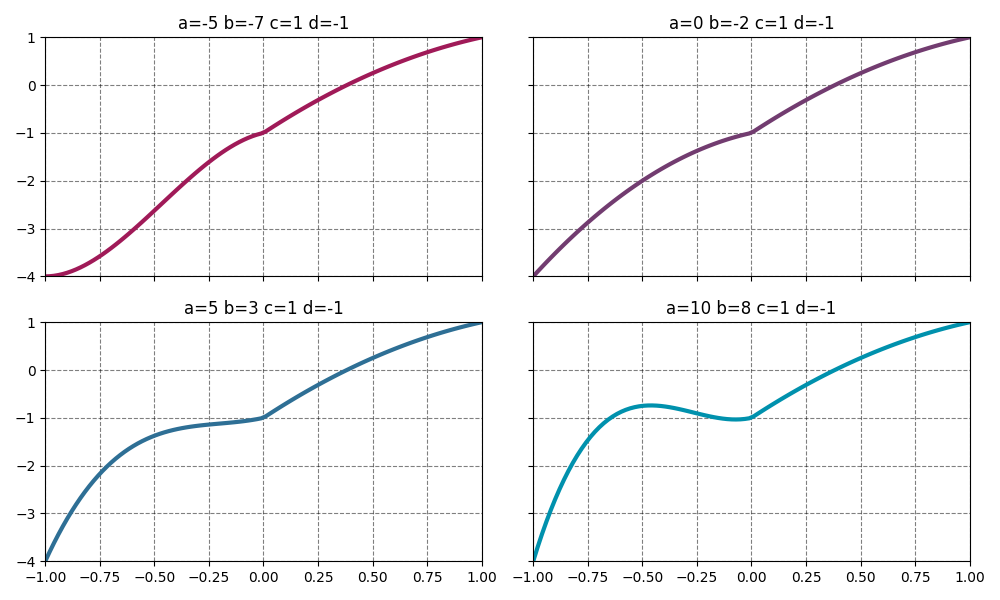
\includegraphics[width=14cm]{Graphics/problema02a.png}
              \caption{Función $f$ con varios parámetros.}
              \label{fig:problema02a}
          \end{figure}

    \item Determina los valores de $a,b,c,d$ si $f$ interpola $f'(-1)=6$ y $f(1)=-1$.

          Calculando la primer derivada de $f$, se obtiene lo siguiente:

          \begin{equation*}
              f'(x) = \begin{cases}
                  f'_0(x)= 3ax^2+2bx+c & -1\leq x \leq 0 \\
                  f'_1(x) = 2d(x-1) +c & 0\leq x \leq 1
              \end{cases}
          \end{equation*}

          Como $f'$ debe de ser continua, entonces $f'_0(0) = f'_1(0)$. Contemplando las condicones dadas, entonces se obtiene el siguiente sistema de ecuaciones:

          \begin{align*}
              3a -2b +c & =6  \\
              c         & =-1 \\
              -2d +c    & c
          \end{align*}

          Por lo tanto, se obtiene que la solución del sistema de ecuaciones es:

          \begin{align*}
              a & \in \Re          \\
              b & = \frac{3a-7}{2} \\
              c & =-1              \\
              d & = 0
          \end{align*}

          Se obtiene que el parámetro $a$ es un parámetro libre, entonces este puede tomar cualquier valor. Para observar su comportamiento se evaluo con los valores de $\{-5,0,5,10\}$. En la figura \ref{fig:problema02b} se muestra la función $f$ con los parámetros obtenidos.
          \begin{figure}[H]
              \centering
              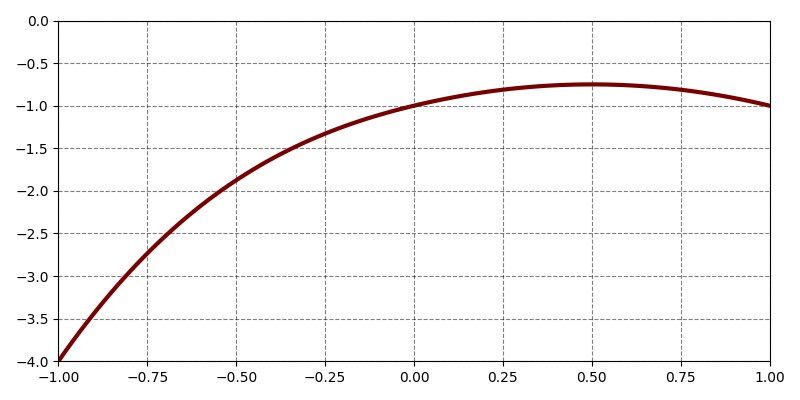
\includegraphics[width=14cm]{Graphics/problema02b.png}
              \caption{Función $f$ con varios parámetros.}
              \label{fig:problema02b}
          \end{figure}
\end{enumerate}
\pagebreak